% GigaScience template
\documentclass[a4paper,num-refs]{oup-contemporary}

%%% Journal toggle; only specific options recognised.
%%% (Only "gigascience" and "general" are implemented now. Support for other journals is planned.)
\journal{gigascience}

\usepackage{graphicx}
\usepackage{siunitx}
\papercat{Paper}

%%%% Packages %%%%

\usepackage{minted} % Used for JSON highlighting
\usepackage{pdfcomment} % Used for notes and todos
\usepackage{algorithm} % Algorithm float
\usepackage{algpseudocode} % Algorithmic environment
\usepackage{xspace}

%%%% Commands %%%%

\newcommand{\note}[2]{\pdfmargincomment[color=yellow,author=#1,open=true]{#2}}
\newcommand{\todo}[1]{\color{red}TODO: #1\color{black}}
\newcommand{\boutiques}{Boutiques\xspace}
\newcommand{\notimplementedyet}[1]{\color{blue}\emph{#1}\footnote{Still needs to be implemented}\color{black}\xspace}
\algrenewcommand{\algorithmiccomment}[1]{\# \textit{#1}} % so that comments in algorithms are preprended by '#' instead of a small right arrow

\title{Boutiques: a flexible framework for automated application integration in computing platforms}

\begin{document}

\author[1]{Tristan Glatard}
\author[2,3]{Gregory Kiar}
\author[2,3]{Tristan Aumentado-Armstrong}
\author[2,3]{Natacha Beck}
\author[4]{Pierre Bellec}
\author[2,3]{R\'emi Bernard}
\author[5]{Axel Bonnet}
\author[5]{Sorina Camarasu-Pop}
\author[5]{Fr\'ed\'eric Cervenansky}
\author[2,3]{Samir Das}
\author[6]{Rafael Ferreira da Silva}
\author[7]{Guillaume Flandin}
\author[5]{Pascal Girard}
\author[8]{Krzysztof J. Gorgolewski}
\author[9]{Charles R.G. Guttmann}
\author[1]{Val\'erie Hayot-Sasson}
\author[4]{Pierre-Olivier Quirion}
\author[2,3]{Pierre Rioux}
\author[10]{Marc-\'Etienne Rousseau}
\author[2,3]{Alan C. Evans}

\affil[1]{Department of Computer Science and Software Engineering, Concordia University, Montreal, Canada}
\affil[2]{McGill University, Montreal, Canada}
\affil[3]{Montreal Neurological Institute, Montreal, Canada}
\affil[4]{Centre de Recherche de l'Institut de G\'eriatrie de Montr\'eal CRIUGM, Montréal, QC, Canada}
\affil[5]{University of Lyon, CNRS, INSERM, CREATIS, Villeurbanne, France}
\affil[6]{University of Southern California, Information Sciences Institute, Marina del Rey, CA, USA}
\affil[7]{Wellcome Trust Centre for Neuroimaging, London, UK}
\affil[8]{Department of Psychology, Stanford University, Stanford, California, USA}
\affil[9]{Center for Neurological Imaging, Department of Radiology, Brigham and Women's Hospital, Boston, Massachusetts, USA}
\affil[10]{Compute Canada}

\begin{frontmatter}
\maketitle

\begin{abstract}
We present \boutiques, a system to automatically publish, integrate
and execute applications across computational platforms. \boutiques
applications are installed through software containers described in a
rich and flexible JSON language. A set of core tools facilitate the
construction, validation, import, execution, and publishing of
applications. \boutiques is currently supported by several distinct virtual
research platforms, and it has been used to describe dozens of
applications in the neuroinformatics domain. We expect \boutiques to
improve the quality of application integration in computational
platforms, to reduce redundancy of effort, to contribute to computational
reproducibility, and to foster Open Science.
\end{abstract}

\begin{keywords}
Application integration; Containers; Neuroinformatics.
\end{keywords}
\end{frontmatter}

\section{Introduction}

Computational platforms such as web services, portals, scientific
gateways, workflow engines and virtual research environments commonly
integrate third-party applications to enable various types of data
processing. Applications, however, are often manually and
repeatedly integrated whereas automating and
sharing this effort would improve computational
reproducibility~\cite{peng2011reproducible,Stodden1240} and contribute
to Open Science. Meanwhile, container systems such as
Docker\footnote{\url{https://www.docker.com}} and
Singularity~\cite{kurtzer2017singularity} have emerged to facilitate
the sharing and migration of software by defining immutable, reusable
execution environments.

We present \boutiques, a system to publish, integrate and execute
command-line applications across platforms (see
Figure~\ref{fig:diagram}).  In \boutiques, a command line is described
using a flexible template comprising the inputs it requires and the
outputs it produces. Inputs may be passed directly on the command line
or through configuration files. They may also be inter-dependent, for
instance mutually exclusive. Such formal descriptions, simply referred
to as \emph{descriptors}, link to a container image where the given
application is installed. \boutiques descriptors allow for automatic
application integration in platforms, and advanced validation of input
values to prevent errors.  \boutiques descriptors are intended to be
produced by scientific application developers, stored alongside their
application, indexed by common repositories, and consumed by execution
platforms.  A set of core tools facilitate the construction,
validation, import, execution, and publishing of \boutiques
descriptors.

The remainder of this paper describes the \boutiques system
and reports on its adoption by platforms
and applications in the neuroinformatics domain, our primary field of
interest. It closes on a discussion and
comparison with related systems.

\begin{figure}
  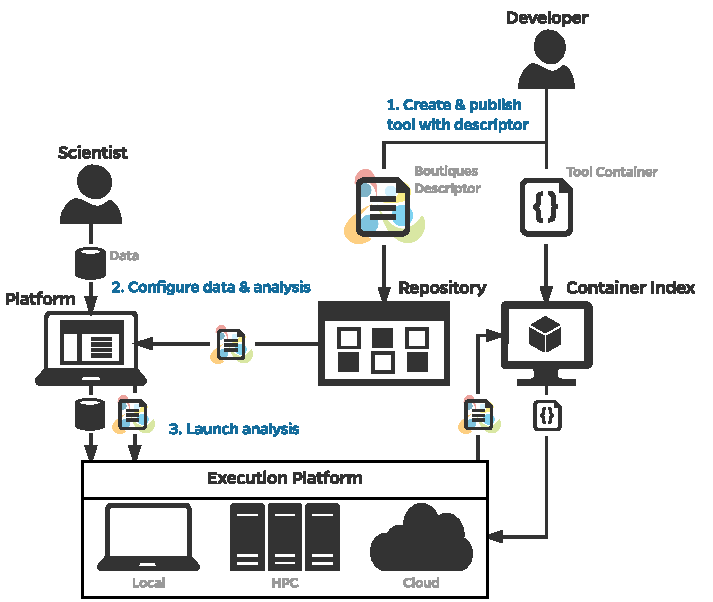
\includegraphics[width=\columnwidth]{boutiquesfig1.pdf}
  \caption{Publication, integration and execution of applications with \boutiques.}
  \label{fig:diagram}
\end{figure}

%% Application integration consists of 1)~installing the application
%%   on the target infrastructure, 2)~describing the application in a
%%   format compatible with the execution platform, and 3)~generating
%%   proper user interfaces. 

\section{System description}

In \boutiques, applications are described with a JSON descriptor that
specifies the command-line template, inputs and outputs. The
descriptor may point to a container where the application and all its
dependencies are installed. It may also contain an invocation schema
used for input validation (this will be created at runtime if it is
not found). At runtime, the execution platform builds the command line
from the descriptor and the values entered by the user. The platform runs
the command line on the execution infrastructure, e.g., a server, a
cluster or a cloud, within a container whenever available. To build
and run the command line, the platform may rely on the \boutiques core
tools, in particular the validator and executor, packaged through the
\texttt{bosh} command-line utility.

\subsection{Command-line description}

The core component of the descriptor is a command-line template
complying to the syntax of the \texttt{bash} UNIX shell, the default
shell on most of the Linux distributions and on OS X. The command-line
template is a single string that may contain placeholders for input and output values, called
value keys. It may also encompass several commands separated by
\texttt{bash} constructs such as semicolons, pipes (\texttt{|}) or
ampersands (\texttt{\&}), to facilitate the embedding of basic
operations on the command line, for instance directory creation, input
decompression or output archival.

Here is an example of a typical command-line template:
\begin{verbatim}
exampleTool_1 [CONFIG_FILE] [STRING_INPUT] [FILE_INPUT]  | \
  exampleTool_2 [FLAG_INPUT] [NUMBER_INPUT] >> [LOG].txt
\end{verbatim}
The template contains five value keys, identified by square brackets,
that will be replaced by values and file names according to the user
input when the application is executed. Flags will also be added
wherever appropriate, with customizable separators. Value keys have to
be unique but do not have to comply to any particular syntax. Note the
use of the \texttt{|} operator to chain applications, and of
the \texttt{>>} operator to redirect the standard output to a file.

\subsection{Input description}

\paragraph{General properties} Inputs must have a name, a unique
identifier, and a type. They may be optional, have a description, a
value key, a flag and flag separator, and a default value. Inputs may
also be ordered lists: in this case, value keys are substituted by the
space-separated list of input values.

\paragraph{Types} Inputs may be of type \texttt{String}, \texttt{Number},
\texttt{Flag} or \texttt{File}. \texttt{File} may also represent a directory.
Types can be restricted to a specific set of values or to a specific range.

\paragraph{Groups and dependencies} Groups of inputs may be defined
with an identifier, name, and list of input identifiers. Groups may be
used to improve the presentation in a graphical user interface, and to
specify the following constraints among inputs:
(1)~\texttt{mutually-exclusive}: only one member in the group may have
a value; (2)~\texttt{one-is-required}: at least one member in the
group must have a value; (3)~\texttt{all-or-none}: if any of the
members have a value then all members must have a value. Dependencies among
inputs may also be defined regardless of a particular group: an input
may (1)~require a list of inputs and (2)~disable a list of inputs.

Listing~\ref{listing:input-example} shows the definition of an input in the
command line exemplified above. According to this definition and assuming
that the input value entered by the user is 0.3, the string
\texttt{[NUMBER\_INPUT]} will be replaced by \texttt{-n=0.3} on the command
line.
\begin{listing}
\begin{minted}[frame=single,
               framesep=3mm,
               linenos=false,
               xleftmargin=0pt,
               tabsize=4]{js}
{
    "id" : "num_input",
    "name" : "A number input",
    "type" : "Number",
    "value-key" : "[NUMBER_INPUT]",
    "optional" : true,
    "command-line-flag" : "-n",
    "command-line-separator" : "=",
    "minimum" : 0,
    "maximum" : 1,
    "exclusive-minimum" : true,
    "exclusive-maximum" : false
}
\end{minted}
\caption{Example of a \texttt{Number}-type input.} 
\label{listing:input-example}
\end{listing}

\subsection{Output description}

Application outputs are files and directories that need to be
delivered to the user once the execution is
complete. Outputs need to be specified so that computing platforms can
identify the files that must be saved after the execution and raise
errors if they are not present.

In \boutiques, output files must have a unique identifier, a name, and
a path template that specifies the file or directory name. Path
templates may include input value keys in case output files are named
after the input values. In this case, input values may be stripped
from specific strings, e.g., file extensions, before being substituted
in the path template. Output files may also have a description, a
command-line flag, a flag separator, and a value key in case they
appear on the command line. They may be optional in case the file is
not always produced by the application, for instance when it is
produced only when a particular flag is activated. They may also be
lists: in this case, the path template must contain a
wildcard (\texttt{*}) matching any string of characters and defining
the pattern used to match the output files in the list.

Listing~\ref{listing:output-example} shows the definition of an output
file in the command line exemplified before. According to this
definition and assuming that the string input value entered by the
user is \texttt{foo.csv}, the string \texttt{[LOG]} will be
replaced by \texttt{log-foo} on the command line.

\begin{listing}
\begin{minted}[frame=single,
               framesep=3mm,
               linenos=false,
               xleftmargin=0pt,
               tabsize=4]{js}

{
  "id": "logfile",
  "name": "Log file",
  "description": "The output log file",
  "path-template": "log-[STRING_INPUT]",
  "value-key": "[LOG]",
  "path-template-stripped-extensions": [".txt", ".csv"],
  "optional": false
}
\end{minted}
\caption{Example of an output leveraging \texttt{path-template} search-and-replacement.} 
\label{listing:output-example}
\end{listing}

\subsection{Configuration files}

A large number of applications rely on configuration files rather than
command-line options to define their input and output parameters. As
the number of parameters increases, command lines rapidly become long
and cumbersome whereas configuration files allow for better structure
and documentation.

Configuration files may be complex though, and specified in any
language.  For this reason, \boutiques allows application developers
to specify their own template containing input and output value
keys. Configuration files are specific types of output files that must
have a file template that defines how
they will be named and where they will be written. They may also have
a value key and a flag in case they need to be passed on the command
line. Listing~\ref{listing:configuration-file-example} shows an
example.
\begin{listing}
\begin{minted}[frame=single,
               framesep=3mm,
               linenos=false,
               xleftmargin=0pt,
               tabsize=4]{js}
{
    "id": "config_file",
    "name": "Configuration file",
    "type": "File",
    "value-key": "[CONFIG_FILE]",
    "path-template": "config.txt",
    "file-template": [
        "# This input is hard-coded",
        "stringInput=foo",
        "# This is an input file",
        "fileInput=[FILE-INPUT]",
        "# And here is the result",
        "fileOutput=[OUTPUT-FILE-NAME]",
        ""
    ]
}
\end{minted}
\caption{Example of a configuration input file. The file template is defined as
  an array of strings to allow for multi-line strings in JSON.}
\label{listing:configuration-file-example}
\end{listing}

\subsection{Command-line construction}

At runtime, a value is assigned to all the mandatory and some of the
optional inputs. %% Inputs of type ``String'' may contain any string,
%% inputs of type "Number" must contain a string representing a number,
%% inputs of type "File" must contain a string representing a file path
%% (absolute or relative to the execution directory) and inputs of type
%% "Flag" must contain a boolean. 
%% When input is a list, the value contains the concatenation of all the
%%values in the list.
%% gk: I agree with not including the above
Algorithm~\ref{algo:command-line} shows how the command line is
constructed from the descriptor and the values entered. It
substitutes all the value keys in the command line, output path
templates and configuration files, and writes the configuration files.
\begin{algorithm}[h!]
\caption{Command-line construction}
\label{algo:command-line}
\begin{algorithmic}
  \State \Comment{Substitute input value keys in output path templates, configuration files and command line.}
  \For{\texttt{input} in \texttt{inputs}}
  \If{\texttt{input} has a \texttt{value-key}}
  \For{\texttt{output} in \texttt{outputs}}
  \State \texttt{stripped\_value} = \texttt{input\_value}
  \If{\texttt{input} type is \texttt{File}}
  \State In \texttt{stripped\_value}, remove  all elements in \texttt{path-template-stripped-extensions}.
  \EndIf
  \State In \texttt{path-template}, replace all occurrences of \texttt{value-key} by \texttt{stripped\_value}.
  \If{\texttt{output} has a \texttt{file-template}}
  \State In any line of \texttt{file-template}, replace all occurrences of \texttt{value-key} by \texttt{stripped\_value}.
  \EndIf
  \EndFor
  \State Prepend \texttt{command-line-flag} and \texttt{command-line-flag-separator} to \texttt{input\_value}.
  \State In \texttt{command-line}, replace all occurrences of \texttt{value-key} by \texttt{input\_value}.
  \EndIf
  \EndFor

  \State \Comment{Substitute output value keys in configuration files and command line.}
  \For{\texttt{output} in \texttt{outputs}}
  \If{\texttt{output} has a \texttt{value-key}}
  \For{\texttt{output} in \texttt{outputs}}
  \If{\texttt{output} has a \texttt{file-template}}
  \State In any line of \texttt{file-template}, replace all occurrences of \texttt{value-key} by \texttt{path-template}.
  \State \Comment{Input \texttt{value-key} have been substituted in \texttt{path-template} previously.}
  \EndIf
  \EndFor
  \State Prepend \texttt{command-line-flag} and \texttt{command-line-flag-separator} to \texttt{path-template}.
  \State In \texttt{command-line}, replace all occurrences of \texttt{value-key} by \texttt{path-template}.
  \EndIf
  \EndFor

  \State \Comment{Write all configuration files.}
  \For{\texttt{output} in \texttt{outputs}}
  \If{\texttt{output} has a \texttt{file-template}}
  \State Write \texttt{file-template} in \texttt{path-template}
  \State \Comment{Value keys have been substituted in \texttt{file-template} previously.}
  \EndIf
  \EndFor

\end{algorithmic}
\end{algorithm}

\subsection{Invocation schema}

Rigorous input validation is an important motivation for
\boutiques. For this purpose, \boutiques relies on an
application-specific JSON schema, called \emph{invocation schema}, to
specify the input values accepted by an application. Platforms can
rely on invocation schemas to validate inputs using
any JSON validator, without having to develop specific code.

Invocation schemas, however, are complex JSON objects. Basically, they
must represent the properties described above in a formal way,
including dependencies between
inputs. Listing~\ref{listing:invocation-schema-example} shows an
example of how dependencies between mutually exclusive parameters are
defined in the invocation schema. To relieve application developers
from the burden of having to write JSON schemas, invocation
schemas can be generated automatically by the \texttt{bosh}
command-line utility. The invocation schema is stored as an optional
property of the \boutiques descriptor.

%% \notimplementedyet{The invocation schema also has a
%%  \texttt{task-dependencies} array that allows specifying that the new
%%  invocation may start only when previously-submitted invocations have
%%  completed. This property is used in the parallelization model
%%  described hereafter.}

\begin{listing}
\begin{minted}[frame=single,
               framesep=3mm,
               linenos=false,
               xleftmargin=0pt,
               tabsize=4]{js}
{
  "dependencies" : {
      "num_input" : {
         "properties" : {
            "str_input" : {
               "not" : {}
            }
         }
      },
      "str_input" : {
         "properties" : {
            "num_input" : {
               "not" : {}
            }
         }
      }
   }
}
\end{minted}
\caption{Excerpt from invocation schema showing dependencies between
  two mutually exclusive parameters \texttt{num\_input} and
  \texttt{str\_input}.}
\label{listing:invocation-schema-example}
\end{listing}

%% \subsection{Parallelization support}
%% \label{sec:parallelization}
%% \boutiques supports parallelism by allowing applications to submit new
%% invocations through \notimplementedyet{the following protocol}:
%% \begin{enumerate}
%% \item Applications write a JSON object complying to the invocation
%%   schema in their execution directory.
%% \item The platform reads the JSON object, creates the corresponding
%%   invocation, and writes back the invocation id in the same directory.
%% % The platform could also support status requests.
%% \end{enumerate}
%% Several invocations can be submitted at once, possibly using the
%% \texttt{task-dependencies} array to specify dependencies among
%% them. This mechanism is implemented in the Boutiques schema using a
%% single property, \texttt{can-submit-tasks}.

%% Although very simple, this model allows wrapping complete
%% workflows. Workflows are wrapped as any other application, and they
%% can be executed using any engine provided that it is installed in the
%% container image referred in the application descriptor. 

\subsection{Workflow support}

\boutiques does not specify a particular language to build workflows
from descriptors, due to the large amount of specialized frameworks to
do so. However, workflows can be both composed from and described as
\boutiques descriptors: workflow engines can leverage the
\texttt{bosh} tools to call \boutiques applications from their
descriptors; in turn, workflows can be described as \boutiques
descriptors. Such a ``task encapsulation'' model allows for a scalable
and reliable execution of workflows expressed in a variety of
languages, as detailed in ~\cite{GLATARD2017239}.

\subsection{Containers}

Applications may be installed in a container image complying to the
Docker, Singularity or rootfs format. We intentionally support
multiple container formats as we anticipate that they will be used for
different purposes. For instance, Docker is well suited for developers
and users who manipulate applications on their local workstations or
the cloud. It is well documented, maintained and it has a rich
ecosystem of tools to build and run containers on most operating
systems. Singularity is more suited for users and platforms that need
to run applications on shared computing clusters. Bridges exist among
these containers formats to convert container images across
frameworks. For instance, a platform dedicated to high-performance computing may accept
descriptors referring to Docker containers to facilitate application
integration by developers, and run these images on clusters using
Singularity.

Container images are defined from their URL (rootfs) or image name in
a Docker or Singularity index. Descriptors may specify a working
directory where the application has to be run, they may indicate if
the image has an entry point, and they may also report a hash to
accurately identify container images and detect updates.

Containers were adopted because they allow for an automated and
lightweight integration of application implementations in
platforms. They are extremely useful to improve the reproducibility of
analyses as variations in the software environment may have an
important impact on the computed results. They also have limitations,
in particular they do not specify the hardware architecture required
to execute an application, which can be an issue in some cases.

%%Containers are not mandatory though. If an application descriptor does
%%not contain any reference to a container, the platform will assume
%%that the application is pre-installed on the execution infrastructure. 
%% gk: I believe we only support containers now, correct?

\subsection{Resource requirements}

\boutiques descriptors may contain requirements regarding the number
of CPU cores or nodes, the amount of RAM or disk storage, and the
total walltime expected for a typical execution of the
application. Such properties are called ``suggested resources'' as we
are well aware that the actual resource requirements usually depend on
the input data, parameters and hardware infrastructure.


\subsection{Custom properties}

Custom properties may be added to the Boutiques specification without
restriction. Custom properties are grouped together in a specific JSON object
to facilitate validation. They may be useful to implement
platform-specific features but they should be used with care to avoid
making applications dependent on a particular platform or replacing
existing functionality already represented in the \boutiques schema.

\subsection{Core tools} 

\boutiques is available on Python through the PyPi package repository
as ``\texttt{boutiques}''. The \boutiques package exposes a
command-line utility to the user, \texttt{bosh}, which contains
entrypoints for all core functions within \boutiques. The core tools
provided by \boutiques are, the: validator, executor (for both launch
and simulation), invocation schema handler, importer, and
publisher. The tools exposed through the command-line interface are also
available consistently through a Python API by importing the
\boutiques package. Though not a component of the \boutiques tool
chain, a Jupyter Notebook tutorial exists to facilitate new users
getting started with \boutiques.

\paragraph{Validator} The \boutiques validator checks conformance of JSON
descriptors to the \boutiques schema using a basic JSON validator. It
also performs the following checks that cannot be easily implemented
in JSON schema: value keys are unique among inputs, input and output
identifiers are unique, input and output value keys are all included
in the command line, identifiers with the same value key are mutually
exclusive, value keys are not contained within each other (which would
puzzle substitution), output path templates are unique (to avoid
results to overwrite each other), inputs of type Flag have a
command-line flag, are optional and are not lists, the default value
of restricted types is part of the restriction, an input cannot both
require and disable another input, required inputs cannot require or
disable other parameters, group member identifiers must correspond to
existing inputs and cannot appear in different groups, mutually
exclusive groups cannot have members requiring other members,
one-is-required groups should never have required members, and
all-or-none group members must not be required.


\paragraph{Executor} The executor has two modes of operation: \emph{simulate} and \emph{launch}. The simulate mode can generate hypothetical command lines from
random values given the descriptor (and corresponding invocation
schema) for debugging purposes, or display the command that would be
executed given a provided valid invocation. The launch mode can
execute command line from a \boutiques descriptor and a set of input
values represented in JSON file complying with the invocation schema.
It runs the command in a container provided that the required
framework (e.g. Docker) is installed. The executor can be used
by application users to run applications locally, or by platforms to
generate command lines to be run on the execution infrastructure.

\paragraph{Invocation Schema Handler} The invocation schema handler can create an
invocation schema from a \boutiques descriptor and validate input data
against it using a regular JSON validator. It can be used to add
invocation schemas to existing descriptors. It is used by the executor
if no invocation schema is present in the \boutiques descriptor being
deployed.

\paragraph{Importer} The importer takes \boutiques descriptors from older versions and
updates them to be compliant with the most recent version of the schema. This tool can
also create descriptors from selected application collections, such as BIDS
apps~\cite{gorgolewski2017bids}.

\paragraph{Publisher} As \boutiques has primarily been adopted in the neuroinformatics
community, the publisher gets a further description (such as author,
website, etc.) of the described application, and adds an index to it
on
NeuroLinks\footnote{\url{https://brainhack101.github.io/neurolinks}},
a repository containing links to neuroinformatics resources and
tools. This functionality could be extended to new repositories for
other domains, such as Bioconductor for
bioinformatics~\cite{gentleman2004bioconductor}.

\section{Results}

\subsection{Supported platforms}

The import and execution of \boutiques applications is currently
supported in the platforms enumerated below.

\subsubsection{CBRAIN}

CBRAIN (\url{http://github.com/aces/cbrain}) ~\cite{SHER-14} is a web
platform to process data distributed into multiple storage
locations on computing clusters and clouds. CBRAIN offers transparent
access to remote data sources, distributed computing sites, and an
array of processing and visualization tools within a controlled,
secure environment.  The CBRAIN service deployed at the Montreal
Neurological Institute relies on the infrastructure provided by
Compute Canada~\cite{das2016mni}. It currently provides 500+
collaborators in 22 countries with web access to several systems,
including 6 clusters of the Compute Canada high-performance computing
infrastructure (totaling more than 100,000 computing cores and 40~PB of
disk storage) and Amazon EC2. CBRAIN transiently stores about 10
million files representing over 50~TB distributed in 42 servers. 51
public data processing applications are integrated and over 340,000
processing batches have been submitted since 2010.

Applications in CBRAIN are integrated as Ruby classes that create web
forms, validate parameters and run command lines on computing
resources. \boutiques is supported through a set of templates that
generate such classes from the application descriptor. Two application
integration modes are available:
\begin{enumerate}
  \item The descriptor is stored in a CBRAIN plugin and the Ruby
    classes are generated on-the-fly when CBRAIN starts. This mode
    allows CBRAIN developers to update all \boutiques applications at
    once by editing the templates. However, it does not allow for
    customization beyond the \boutiques schema. To provide more
    flexibility, we added a custom property
    (\texttt{cbrain:inherits-from-class}) to the \boutiques descriptor
    to define the Ruby class that should be used as parent class for
    the application.
  \item Ruby classes are generated from descriptors
    through an offline process and integrated in CBRAIN as any other
    application. This mode allows developers to customize applications
    by editing the generated Ruby classes, but the resulting
    applications are difficult to maintain in the long term, in
    particular when the descriptors are updated.
\end{enumerate}

We also extended CBRAIN to enable the parallelization of workflows
wrapped as \boutiques descriptors. Applications with the
\texttt{cbrain:can-submit-new-tasks} custom property may submit sub-tasks by
creating \boutiques invocations in their working directory. CBRAIN
periodically scans working directories, submits the requested
sub-tasks, and writes back an invocation identifier in the same
directory. This parallelization model is simple, the application only
needs to write \boutiques invocations and communication happens
through the file system, and it is also powerful as it enables the
parallelization of complex workflows such as the Niak ones
described later. 

We also introduced a new list mechanism in CBRAIN to facilitate the
iteration of \boutiques applications on large sets of files. CBRAIN
lists are specific files that contain references to other CBRAIN
files. When a list is passed to a \boutiques application, the elements
in the list are either concatenated in a single command line (when the
corresponding \boutiques input is a list), or a new command line is
generated for every element in the list (when the input is not a
list). Supporting lists as a specific CBRAIN file type allows for
improved validation. For instance, lists that contain references to
non-existent or deleted files can be detected. It also allows users to
edit lists using their own tools such as scripts or spreadsheet
applications.

\subsubsection{Nipype}
Nipype
(\url{http://nipype.readthedocs.io/en/latest})~\cite{gorgolewski2011nipype}
is a workflow engine widely used in neuroinformatics. Nipype workflows
can be composed from \boutiques applications using the Python API. As
an example, we implemented
NipBIDS\footnote{\url{https://github.com/big-data-lab-team/sim/tree/master/sim/other_wf_examples/nipype}},
a Nipype workflow to process BIDS datasets using BIDS apps imported as
\boutiques applications. NipBIDS iterates participant analyses on all
the subjects found in a BIDS dataset and runs a group analysis if
requested.

\subsubsection{SPINE}
SPINE (\url{http://spinevirtuallab.org}), which stands for Structured
Planning and Implementation of New Explorations, is a web-based,
collaborative platform (virtual laboratory) designed to support the
design and execution of experiments centered on specific scientific
questions.  SPINE enables distributed data collection and management,
as well as experiment design, execution, and review. Boutiques will serve
as SPINE's algorithm and workflow repository, and enables unequivocal
referencing of specific workflows applied to specified datasets within
an experiment, thereby describing the provenance and facilitating the
reproducibility of image-derived measurements. Workflows in SPINE may
combine human image annotation with automated image processing
algorithms. Future development will focus on extending Boutiques
workflow descriptors to include the identification and
characterization of human operators and their specific historic
performance on the required tasks. SPINE is currently hosted at
Brigham \& Women's Hospital in Boston, and supports several
international projects.

\subsubsection{VIP}

The Virtual Imaging Platform (VIP)~\cite{GLAT-13} is a web portal for
medical simulation and image data analysis. VIP makes applications
available as services, and connects them to the biomed Virtual
Organization (VO) in the European Grid
Infrastructure\footnote{\url{https://www.egi.eu}}. The biomed VO
interconnects approximately 65 computing sites world-wide and provides
access to 130 computing clusters and 5~PB of storage.  The VIP service
is deployed at the Creatis
laboratory\footnote{\url{https://www.creatis.insa-lyon.fr}} in Lyon
and it uses the DIRAC French national
service\footnote{\url{https://dirac.france-grilles.fr}} to execute
jobs on EGI grid and cloud resources.  As of October 2017, VIP counts
more than 1,000 registered users and a growing number of available
applications.

Until recently, applications were manually integrated in VIP as
workflows written in the Gwendia~\cite{MONT-09} language and executed
with the MOTEUR~\cite{GLAT-08} engine.  As of today, Boutiques is
supported through an importer tool that parses the JSON descriptor and
automatically generates the corresponding application workflow and the
wrapper script that handles, among other things, the execution of the
command line.  In VIP, application workflows enable (1) iterations on
input lists, (2) the generation of parallel tasks, and (3) the
concatenation of multiple applications. For example, the applications
used in the MICCAI challenges described below required workflows to
evaluate results using the metrics defined by the
challenge. Application concatenation is handled at the importer level
based on pre-defined workflow templates.

\subsection{Integrated applications}

% cbrain-plugins-neuro

%%Table~\ref{table:applications} summarizes the applications described
%%with \boutiques and the main features used.

Dozens of neuroinformatics applications were integrated in CBRAIN or
VIP using \boutiques. The main ones are described below. Several
\boutiques descriptors were published in Neurolinks through the
\texttt{bosh} publisher.



%% \paragraph{Nipype} We instrumented the Nipype workflow engine~\cite{gorgolewski2011nipype} 
%% to export the applications described in its internal Python
%% description language to \boutiques. \todo{Update nipype\_cmd to
%%   support the latest \boutiques schema and complete this paragraph.}

\subsubsection{Anatomical imaging}

\paragraph{FSL} Several MRI analysis applications from the FMRIB Software
library (FSL~\cite{jenkinson2012fsl}) were integrated in CBRAIN using
\boutiques: BET, fsl\_anat, FAST and FIRST. Descriptors are
on Neurolinks.

\paragraph{Anima}
\texttt{animaN4BiasCorrection}, an ITK-based bias field correction application from the
Anima\footnote{\url{https://github.com/Inria-Visages/Anima-Public/wiki}}
project was made available in VIP through \boutiques. 

\subsubsection{Functional MRI (fMRI)}

\paragraph{Niak} The Niak fMRI pre-processing pipeline~\cite{bellec2011neuroimaging}, executed with the Pipeline System
for Octave and Matlab (PSOM)~\cite{bellec2012pipeline}, was integrated
in CBRAIN through \boutiques. The integration uses the CBRAIN
sub-tasking mechanism described earlier so that even the invocations
processing a single subject can be parallelized. It also allows CBRAIN
to leverage the efficient agent model used in PSOM, as described
in~\cite{GLAT-16}. The integration required some work in PSOM to
facilitate its invocation as a non-interactive command-line
application. The resulting CBRAIN plugin is available at
\url{https://github.com/SIMEXP/cbrain-plugins-psom}.  Descriptors
are on Neurolinks.

\paragraph{GinFizz}
We integrated the
GinFizz\footnote{\url{https://github.com/thomashirsch/ginfizz}}
Nipype-based fMRI pre-processing pipeline in VIP with \boutiques.  A
few technical issues coming from the management of users in Docker
containers had to be addressed: to enable the execution in \boutiques
we had to override the permissions of files and folders in the GinFizz
container. We also had to install all the GinFizz pipeline components
in a single container while multiple ones were used by the application
initially.

%% Ginfizz performs multiple
%% preprocessing steps and basic analyses such as: (i) realignment
%% (motion registration and correction), (ii) slice timing (temporal
%% interpolation to correct for the delay of acquisition between slices),
%% (iii) coregistration (registering functional and structural data),
%% (iv) normalization (registering of functional and anatomical data to a
%% match a template that has to be specified), and (iv) smoothing
%% (spatial filtering to increase Signal to Noise ratio).

\subsubsection{Diffusion imaging}

\paragraph{MRTrix3}
A few applications from the MRtrix3
package~\cite{tournier2012mrtrix}\footnote{\url{http://www.mrtrix.org/}} for diffusion MRI processing were also made available in VIP,
as well as a pipeline developed at Creatis, which combines MRtrix3 and
FSL applications.

\paragraph{ndmg} The NeuroData MRI to Graphs one-click connectome estimation
pipeline~\cite{kiar2017comprehensive}, developed in Python and leveraging FSL, was
exported to \boutiques and is available at \url{https://github.com/neurodata/boutiques-tools}.
The ndmg pipeline is deployed in CBRAIN via its \boutiques descriptor, and is available
both through Docker and Singularity container environments.

\subsubsection{Image simulation}

\paragraph{CreaPhase}
The CreaPhase phase-contrast simulator, developed at
Creatis, was integrated in VIP through \boutiques. The inputs had
certain particularities (some needed to be enclosed in simple quotes,
other were vectors of variable size enclosed in brackets) that
required the post-processing of the wrapper script generated by the
\boutiques importer.

\paragraph{ODIN} The Odin MRI simulator~\cite{jochimsen2004odin}\footnote{\url{http://od1n.sourceforge.net}} was integrated
in VIP through \boutiques. Since Odin requires important amounts of
computing resources it is executed by VIP on the EGI grid that
currently does not support Docker. The Docker image was used just for
compilation and testing; the Odin executable was extracted from the
Docker image and the Odin wrapper script was modified accordingly.

\subsubsection{BIDS apps}

BIDS apps~\cite{gorgolewski2017bids}, an effort for the adoption of
the Brain Imaging Data Structure (BIDS) in common neuroimaging
pipelines, require a standardized set of input and output
parameters. We developed a tool as part of the \boutiques importer to
generate a descriptor for any such BIDS app. We validated this tool by
importing BIDS apps containing the Statistical Parametric Mapping
toolbox (SPM)~\cite{penny2011statistical} and the ndmg pipeline
mentioned above. Descriptors are on Neurolinks.


\subsubsection{2016 MICCAI challenges}

We used \boutiques to integrate 23 pipelines in the VIP platform in
the context of two challenges organized by the MICCAI conference in
2016, related to the segmentation of multiple-sclerosis lesions in MR
images (MSSEG
challenge\footnote{\url{https://portal.fli-iam.irisa.fr/msseg-challenge/overview}})
and of tumor volumes in PET images (PETSEG
challenge~\cite{hatt2018}). The
pipelines were integrated in VIP and executed on 205 subjects in a few
weeks only. Some pipelines had to be adjusted manually once integrated in
the platform for the following reasons:
\begin{enumerate}
\item A pipeline
  required a GPU, which we enabled through the
  \texttt{nvidia-docker}\footnote{\url{https://github.com/NVIDIA/nvidia-docker}}
  tool not supported in Boutiques although it could be a possible extension.
\item A pipeline required more than 10 GB of data dependencies (atlas
  data) which exceeded the maximum size allowed for Docker containers
  in our setup. We solved the issue by installing the data in a
  directory of the host server that we mounted in the container.
\item A pipeline wrote more than 10 GB of intermediate data in a
  temporary directory of the container located on a 2 GB partition. We
  solved the issue by mounting a host directory in the temporary directory. 
\end{enumerate}
Two custom properties (\texttt{vip:miccai-challenger-email}
and \texttt{vip:miccai-challenge-team-name}) were also added to the
\boutiques descriptor to help post-process results in the specific
context of MICCAI challenges.


\section{Discussion}
With \boutiques, developers can integrate their applications once and
execute them in several platforms. \boutiques removes the
technological dependency to a particular platform and facilitates
application migration.  Although the motivating use cases were taken
from neuroinformatics, our primary field of interest, nothing prevents
the system from being used in other domains.

\subsection{\boutiques descriptor}

The \boutiques descriptor specification allows describing a wide range
of applications, but it is also getting increasingly complex through
additions such as invocation schemas and dependencies among
inputs. Extending the \boutiques descriptor has two main goals: (1)
validation: incorrect input values and execution results are more
precisely detected when the application descriptor is
comprehensive; (2) automation: a rich descriptor schema reduces the need for
custom application wrappers, which is particularly useful for containerized
applications.

Nonetheless, a complex descriptor schema has a cost for application
developers and platforms, which we address as follows. For developers,
we maintain the set of mandatory descriptor properties as small as
possible so that simple applications can be described in a few lines
only (see Listing~\ref{listing:minimal}). For platforms, we aim at
supporting as many features as possible in the \texttt{bosh} executor
so that only the following steps need to be implemented in a platform,
regardless of the complexity of the descriptor:
\begin{enumerate}
  \item Input entry: generate the interface to enter inputs.
  \item Input validation: create a JSON invocation from the interface,
    validate it against the invocation schema.
  \item Input delivery: transfer the input files to the application
    execution location.
  \item Execution: pass the invocation to the \texttt{bosh} executor to run the application.
  \item Output delivery: from the descriptor, identify the output files
    and deliver them to the user.
\end{enumerate}
In particular, command-line generation and advanced validation
features such as dependencies between inputs are embedded in
\texttt{bosh}, without requiring the platform to support the related
descriptor properties.
\begin{listing}
\begin{minted}[frame=single,
               framesep=3mm,
               linenos=false,
               xleftmargin=0pt,
               tabsize=4]{js}
{
  "name": "echo",
  "tool-version": "1.0",
  "description": "A simple script to test output files",
  "command-line": "echo [PARAM] > output.txt",
  "schema-version": "0.5",
  "inputs": [{
      "id": "param",
      "name": "Parameter",
      "value-key": "[PARAM]",
      "type": "Number"
  }],
  "output-files": [{
      "id": "output_file",
      "name": "Output file",
      "path-template": "output.txt"
  }]
}
\end{minted}
\caption{A minimal \boutiques descriptor.} 
\label{listing:minimal}
\end{listing}

\subsection{Workflow support}

\boutiques intentionally does not provide a workflow language to
compose applications, as this is already possible with numerous
workflow engines. Workflows can be either composed from \boutiques
applications, as we illustrated with the Nipype and MOTEUR engines, or
described as \boutiques applications, as we demonstrated with the Niak
fMRI pre-processing pipeline. Furthermore, the CBRAIN platform has a
sub-tasking mechanism that allows \boutiques applications to submit
tasks, which is used to parallelize workflows wrapped as \boutiques
applications. Based on the CBRAIN experience, we may specify the
sub-tasking mechanism in \boutiques so that other platforms can
benefit from it.  This model is powerful because it shields the
\boutiques specification from specific workflow constructs and it allows
a wide range of workflow engines to be described and used uniformly.


\subsection{Reproducibility}

\boutiques helps computational reproducibility through containers and formal
command-line descriptions. With \boutiques, complete sets of
applications could be easily migrated across execution platforms,
including high-performance computing clusters and individual laptops,
to reproduce analyses. The \boutiques descriptor describes the
parameters and implementation of the application, and the invocation
schema describes the parameter values.

However, reproducibility is a large problem that \boutiques only
partially addresses. At the command-line execution level, containers
help freeze a large fraction of the software ecosystem but they do not
shield against discrepancies arising from different Linux kernel
versions or hardware platforms. For instance, containers may not
execute consistently on different CPUs complying to the x86\_64
architecture (e.g. Intel and AMD) when the application is compiled with
architecture-specific flags such as GCC's \texttt{-march}.

In addition, important runtime parameters, for instance related to
multi-threading or available resources (storage, RAM), may be set by
the execution platform without being specified in the \boutiques
descriptor. Such runtime parameters may impact reproducibility in some
cases. To properly cover this issue, \boutiques descriptors should be
complemented by a provenance framework that captures a detailed trace
of the execution. We plan to leverage the provenance format being
defined by the NeuroImaging Data
Model-Workflow~\cite{ghosh2017capturing} initiative for this purpose.


\subsection{Application types}

So far, \boutiques has focused on the description of non-interactive
command-line applications. While such applications cover a large
fraction of the applications involved in scientific data processing, other
types of programs exist such as web services, interactive applications, and
applications with a graphical user interface (GUI).  Such application
classes could be described in \boutiques through a command-line
mapping. For instance, web services may be wrapped as command-line
applications using tools such as \texttt{curl} or
\texttt{wget}. Interactive applications may also be transformed to
non-interactive ones through configuration files. Finally, nothing
prevents a \boutiques application from popping up a window for a user to
provide input through a GUI. This should, however, be specified
as an extension to the descriptor since most platforms would not support
this feature by default. Graphical output produced by applications
executed in containers should also be treated specifically.

\subsection{Limitations}

A few limitations remain that should be addressed in the
future. First, \boutiques moves the application integration bottleneck
from integration to validation. Using \boutiques, functions can be
automatically exported from frameworks such as Nipype and SPM,
creating hundreds of richly described applications potentially usable
by end-users. However, the automated validation of such applications
remains challenging. A \boutiques-specific testing framework could be
designed and potentially fed by existing frameworks, to address this
issue.

Another limitation is related to the security of containerized
applications. Since containers are usually controlled by application
developers rather than platforms, which is a good thing to reduce
application integration bottlenecks, nothing prevents developers to embed
malicious code in their container at any stage of the process,
possibly after a platform administrator inspected the
container. Containers are bulky file archives that are
cumbersome to inspect. Tools need to be developed to allow for an
easier characterization of container contents, for instance through
comparison digests with respect to validated base images. Singularity
containers have reduced security risks as compared to Docker containers,
but the issue of content transparency is still not avoided.

% How to build modular container images for workflows.

\section{Related work}

Several frameworks have been developed to describe and integrate
applications in various types of platforms. \boutiques focuses on (1)
fully-automatic integration of applications, including deployment on
heterogeneous computing resources through containers, (2)
comprehensive input validation through a strict JSON schema, (3)
flexible application description through a rich JSON
schema.

\subsection{Common Workflow Language}

The Common Workflow Language
(CWL\footnote{\url{http://www.commonwl.org}}) is the work most closely
related to \boutiques as it provides a formal way to describe
containerized applications. In particular, CWL's Command Line Tool
Description overlaps with the \boutiques descriptor. This Section
highlights the main differences between CWL and \boutiques, based on
version 1.0 of the CWL Command Line Tool
Description\footnote{\url{http://www.commonwl.org/v1.0/CommandLineTool.html}}. According
to GitHub, CWL started 6 months before \boutiques (September 2014
vs. May 2015).

\subsubsection{Conceptual differences}

The following differences are conceptual in the sense that they may
not be easily addressed in CWL or \boutiques without deeply
refactoring the frameworks.

First, CWL has a workflow language whereas \boutiques does not. In
\boutiques, workflows are integrated as any other applications, except
that they may submit other invocations to enable workflow
parallelism. This fundamental difference has consequences on the
complexity of CWL application descriptions and on the possibility to
reuse existing workflows in \boutiques. The adoption of ontologies in
CWL may also be another consequence (see below).

CWL imposes a strict command-line format while \boutiques is more
flexible. CWL specifies command lines using an array containing an
executable and a set of arguments whereas \boutiques only uses a
string template. \boutiques' template approach may create issues in
some cases, but it also allows developers to add simple operations to
an application without having to write a specific wrapper. For
instance, a \boutiques command line may easily include input
decompression using the \texttt{tar} command in addition to the main
application command. Importantly, \boutiques' template system allows
supporting configuration files.

CWL uses ontologies while \boutiques does not. Ontologies allow for
richer definitions but they also have an overhead. The main
consequences are the following:
\begin{itemize}
\item CWL uses a specific framework for
validation, called SALAD (Semantic Annotations for Linked Avro Data)
whereas \boutiques uses plain JSON schema. The main goal of SALAD is to
allow ``working with complex data structures and document formats, such
as schemas, object references, and namespaces''. \boutiques only relies
on the basic types required to describe and validate a command line
syntactically. While the use of SALAD certainly allows for
higher-level validation, and may simplify the composition and
validation of complex workflows, it also introduces a substantial
overhead in the specification, and platforms have to use the validator
provided by CWL. On the contrary, a regular JSON validator can be used in \boutiques.
\item  CWL has a rich set of types whereas \boutiques only has simple
types. This may again be seen as a feature or as an overhead
depending on the context. \boutiques tries to limit the complexity of
the specification to facilitate its support by platforms where applications
will be integrated.
\end{itemize}

\subsubsection{Major differences}

The following differences are major but they may be addressed by the
CWL and \boutiques developers as they do not undermine the application
description model.

\begin{itemize}
\item CWL applications have to write in a specific set of directories called
``designated output directory'', ``designated temporary directory''
and ``system temporary directory''. Applications are informed of the location
of such directories through environment variables. Having to write in
specific directories is problematic because applications have to be modified
to enable that. In \boutiques, the path of output files is defined
using a dedicated property.
\item CWL types are richer, not only
semantically but also syntactically. For instance, files have
properties for basename, dirname, location, path, checksum, etc.
\item \boutiques supports various types of containers (Docker,
  Singularity, rootfs) while CWL supports only Docker. Both tools have
  rich requirements: for instance, they may include RAM, disk usage,
  and walltime estimate. CWL has hints, i.e., recommendations that
  only lead to warnings when not respected.
\item In \boutiques, dependencies can be defined among inputs, e.g., to
specify that an input may be used only when a particular flag is
activated. This is a very useful feature to improve validation, in
particular for applications with a lot of options.
\item In \boutiques, named
groups of inputs can be defined, which improves the presentation of
long parameter lists for the user and enables the definition of more
constraints within groups (e.g. mutually exclusive inputs).
\end{itemize}

\subsection{BIDS apps}

BIDS apps~\cite{gorgolewski2017bids} specify a framework for
neuroimaging applications to process datasets complying to the Brain
Imaging Data Structure (BIDS). They share common goals with
\boutiques, in particular reusability across platforms through
containerization. Conceptually, however, BIDS apps and \boutiques are
different since BIDS apps intend to standardize application interfaces
while \boutiques intends to describe them as flexibly as
possible. BIDS apps have a specific set of inputs and outputs, for
instance the input dataset, that have to be present in a specific
order on the command line for the application to be valid. The
specification adopted by BIDS apps simplifies the integration of
applications in platforms as they all comply to the same
interface. However, it is also limited to the subset of neuroimaging
applications that process BIDS datasets and it does not formally
describe application-specific inputs. All in all, BIDS apps and
\boutiques complement each other: BIDS apps provide a practical way to
integrate neuroimaging applications, while \boutiques offers a formal
description of their specific parameters.  \boutiques descriptors can
be generated from BIDS apps using the \texttt{bosh} importer. 

\subsection{Other frameworks}

Several other frameworks have been created to facilitate the
integration of command-line applications in platforms. In
neuroinformatics, many platforms define a formal interface to embed
command-line applications. Among them, the Common
Toolkit\footnote{\url{http://www.commontk.org}} interoperates with
several platforms such as 3D Slicer~\cite{pieper20043d},
NiftyView~\cite{Craddock2016}, GIMIAS~\cite{larrabide2009gimias},
MedInria~\cite{larrabide2009gimias}, MeVisLab~\cite{heckel2009object}
and MITK workbench~\cite{nolden2013medical}. The framework, however,
remains tightly bound to the Common Toolkit's C++ implementation which
limits its adoption, e.g., in web platforms.

In the distributed computing community, systems were also proposed to
facilitate the embedding of applications in platforms. The Grid
Execution Management for Legacy Code Architecture
(GEMLCA~\cite{delaitre2005gemlca}) was used to wrap applications in
grid computing systems. Interestingly, it has been used to embed
workflow engines in the SHIWA
platform~\cite{terstyanszky2014enabling}, in a similar but different
way than proposed by \boutiques.

The recent advent of software containers requires a new generation of
application description frameworks that are independent from any
programming language and that expose a rich set of properties to
describe command lines, as intended by \boutiques.

\section{Conclusion}

\boutiques is available at \url{https://github.com/boutiques}. We
welcome feedback, issue reporting and pull requests. \boutiques adopts
a bottom-up approach where new features are progressively added based
on feedback from applications and platforms. Beyond the technicalities
discussed in this paper, the availability of a solid core of
applications and platforms in the framework is key to its success,
which we plan to continuously enhance.

\section{Acknowledgments}

Pipeline integration for the MICCAI 2016 challenge was funded by the
French National Agency for Research (ANR) through ``France
Life-Imaging''. We also thank Compute Canada and Calcul Québec for
providing a computing infrastructure supporting Docker and Singularity
containers. This research was undertaken thanks in part to funding
from the Canada First Research Excellence Fund, awarded to McGill
University for the Healthy Brains for Healthy Lives initiative. We also
thank the developers of all the applications described with \boutiques.

\bibliography{biblio}

\end{document}
